\documentclass[letterpaper,12pt,fleqn]{article}
\usepackage{matharticle}
\usepackage{pgfplots}
\pgfplotsset{compat=1.14}
\pagestyle{plain}
\begin{document}

\begin{center}
\Large Math-19 Homework \#7 Solutions
\end{center}

\vspace{0.5in}

Submit this homework on this page.

\underline{Problems}

Use the graph of $y=f(x)$ to answer the following questions:

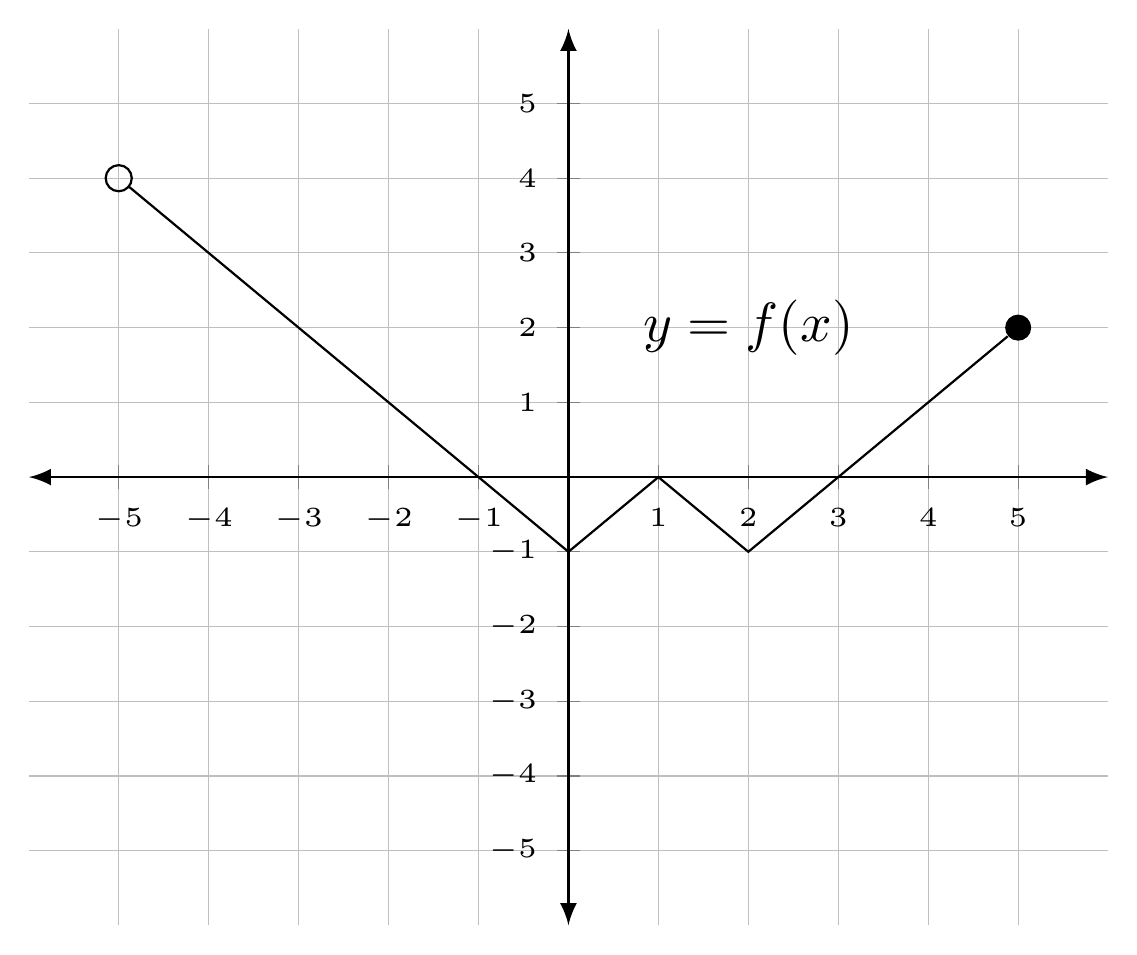
\begin{tikzpicture}[scale=2]
  \begin{axis}[
      xmin=-6,xmax=6,
      ymin=-6,ymax=6,
      grid=both,
      grid style={line width=.1pt, draw=gray!10},
      major grid style={line width=.2pt,draw=gray!50},
      axis lines=middle,
      axis line style={latex-latex},
      xtick={-5,-4,-3,-2,-1,0,1,2,3,4,5},
      ytick={-5,-4,-3,-2,-1,0,1,2,3,4,5},
      ticklabel style={font=\tiny},
    ]
    \node (a) [circle,draw,scale=0.5] at (-5,4) {};
    \node (b) [circle,fill,scale=0.5] at (5,2) {};
    \draw (a) to (0,-1) to (1,0) to (2,-1) to (b);
    \node at (2,2) {$y=f(x)$};
  \end{axis}
\end{tikzpicture}

\begin{enumerate}
\item What is $f(2)$?

  $f(2)=-1$

\item What is the y-intercept?

  $(0,-1)$

\item For what values of $x$ is $f(x)=0$?

  $x=-1,1,3$

\item What is the domain of $f$, in interval notation?

  $(-5,5]$

  \newpage

\item What is the range of $f$, in interval notation?
  
  $[-1,4)$

\item On what intervals is $f$ increasing?

  $[0,1]$ and $[2,5]$

\item On what intervals is $f$ decreasing?

  $(-5,0]$ and $[1,2]$

\item What are the local minima (if any)?

  $(0,-1)$ and $(2,-1)$

\item What are the local maxima (if any)?

  $(1,0)$ and $(5,2)$

\item What is the absolute maximum (if any)?

  none.
  
\end{enumerate}

\end{document}
